discrepancies \documentclass[11pt, letterpaper]{article}
\usepackage[margin=1.25in,  marginparwidth=2.5cm, marginparsep=0.25cm]{geometry}

% \setlength{\textheight}{8.75in}
% \setlength{\oddsidemargin}{.125in}

% \setlength{\textwidth}{6.25in}
% \linespread{1.4}
\usepackage{graphicx}
\usepackage{chemmacros}
\usepackage{amsmath}
\usepackage{float}
\usepackage{gensymb}
\usepackage{multirow}
\usepackage{color}
\usepackage{wrapfig}
\usepackage{tabularx}
\usepackage{marginnote}
\bibliographystyle{unsrt}
\usepackage[font=small,labelfont=bf]{caption}
\author{N. Belliveau, G. Chure, J. Theriot, R. Phillips}

\begin{document}
\title{Supplemental Information: }
\maketitle

\section{Translation-dependent limits on the rate of cell division.}

Here we consider the hypothesis that the process of translation sets the speed
limit of bacterial growth. We begin by considering the synthesis of the ribosome
itself, finding that it sets a strict limit on division time, and then from there we
consider how the remaining proteome further limits this achievable growth rate.

\subsection{Maximum possible growth rate is set by the time to make a ribosome.}

Ribosomes take a unique position among proteins due to their role in
synthesizing the entire cellular proteome. In order for a cell to maintain its
own pool of ribosomes during division into two daughter cells, a primary
requirement is that the number of ribosomes must be doubled.  Since the  mass of
a single ribosome is about 2.5 MDa, with about 2/3 RNA and 1/3 protein, each
ribosome has to make about 800 kDa of protein. In {\it E. coli},
this corresponds to 7,459 amino acids. At a maximal translation rate of 20 amino
acids per second, this would take just over 6 minutes.  Growing any faster would
result in a drop in the average number of ribosomes as the cell divides and
highlights a strict time limit on how fast a cell can double itself.  This
result is irrespective of the absolute number of ribosomes, and contrasts with
other proteins where the simple solution to making more proteins is to
apparently devote more ribosomes to their synthesis.

\subsection{The translation-limited growth rate is set by the fraction of
ribosomal mass.}

While the inability to parallelize ribosomal synthesis sets an inherent speed
limit, this also represents a somewhat unachievable growth rate since ribosomes must
spend some of their time doubling the remaining proteome. A
translation-limited rate of growth is therefore set by the time to double the
entire proteome. In order to understand the consequence of each ribosome having
to duplicate itself, but also devote time to double the remaining proteome, we
consider a hypothetical cell that consists of only two species of protein:
ribosomes and non-ribosomal proteins. The cell is taken to contain $R$ ribosomes
per cell, and $P$ non-ribosomal proteins per cell. The time $\tau$ needed to
duplicate the entire proteome is simply given by,

\begin{equation}
	\tau = \tau_R + \tau_P,
\label{eq:tau}
\end{equation}
where $\tau_R$ is the time to double the ribosome copy number and $\tau_P$ is the time
required to double the non-ribosomal proteins. While we found that $\tau_R$ is fixed
at about 6 minutes,  $\tau_P$  will depend on the number of ribosomes $R$ available and
can be approximated by,

\begin{equation}
\tau_P = \frac{N_{aa}}{r_t \cdot R}.
\label{eq:tau_P}
\end{equation}
Here $N_{aa}$ refers to the total number of amino acids (aa) that must be
translated, while $r_t$ refers to the elongation rate of translation.
The translation-limited growth rate can then be calculated from,

\begin{equation}
\lambda_{\text{max}} =  \frac{ln(2)} {\tau}.
\end{equation}
Using Equation \ref{eq:tau_P} and \ref{eq:tau}, this becomes,
\begin{equation}
\lambda_{\text{max}} =  \frac{ln(2)} {\tau_R + \frac{N_{aa}}{r_t \cdot R}}.
\label{eq:lambda_max}
\end{equation}
We can see from Equation \ref{eq:lambda_max} that the only way to increase the
translation-limited growth rate would be to make more ribosomes, or if it were
possible, to decrease the number of non-ribosomal proteins. For now we will assume
that the translation elongation rate is fixed at about 20 aa/s but will return to this
assumption in a later section.

let's now use some representative values for $R$ and $N_{aa}$ to calculate
$\lambda_{\text{max}}$. From Schmidt {\it et al.}, cells grown in glucose were
found to have 214 fg of non-ribosomal  protein mass \cite{Schmidt2016}. Taking
the molecular weight of an average amino acid to be 110 g/mol and using Avogadro's number $N_A$, we can estimate
$N_{aa}$ = 214 x 10$^{-15}$g / (110 g/mol) x $N_A$,
which corresponds to about 1x10$^9$ amino acids.  Similarly, we can use their
reported ribosomal mass of about 29 fg to estimate the ribosomal copy number,
$R$. With a molecular weight of about 800 kg/mol as noted earlier,  $R$ =
29 x 10$^{-18}$kg / (800 kg/mol) x $N_A$,   which we find to be about 22,000 per
cell. Using Equation \ref{eq:lambda_max}, this corresponds to a maximum growth
rate of 0.8 hr$^{-1}$, versus the measured rate of 0.58 hr$^{-1}$, suggesting
cells are growing slightly below their maximal rate.

Since the only way to divide faster than this limit set at 0.8 hr$^{-1}$ would be
for the cell to increase the number of ribosomes, we next consider how
growth rate might vary as a function of ribosomal copy number. To
keep our problem simple,  lets first proceed with the simplifying assumption
that our cell consists of  214 fg of non-ribosomal protein, and consider
how $\lambda_{\text{max}}$ varies  as a function of the ribosome copy number $R$
using Equation \ref{eq:lambda_max}.  While in reality we might expect other
proteins to increase in proportion to the number of ribosomes, this calculation
provides us with a bound on the maximum growth rate as a function of $R$.  In
Figure \ref{fig:estimates_translation_toy_1} we consider the range of experimentally observed values
of $R$ from about 10,000 copies per cell to
150,000 copies per cell. One observation is that
the maximum growth rate is always less than that set by the synthesis time of a
ribosome, at about 3 hr$^{-1}$ when $R$ is 150,000 ribosomes per cell. Indeed, while not shown,
we find that $R$ would need to be increased another 10 fold, to
about one million copies per cell, to have a doubling time close to that set by the ribosome (with a 6 minute ribosome synthesis time
corresponding to a growth rate of about 7 hr $^{-1}$).

% One difficultly that
% arises is that in order for a cell to add more ribosomes, it will need to
% increase in size. This might require that other proteins also increase in number to
% maintain a specific proportion relative to the cell size. However,
% that the value of $N_{aa}$ is sufficient to
% build a cell irrespective of the number of ribosomes.
% This in effect provides us with a
% lower bound on the total proteomic content at faster growth rates and a lower
% limit on the achievable growth rate.

\begin{figure}[H]
		\centering
    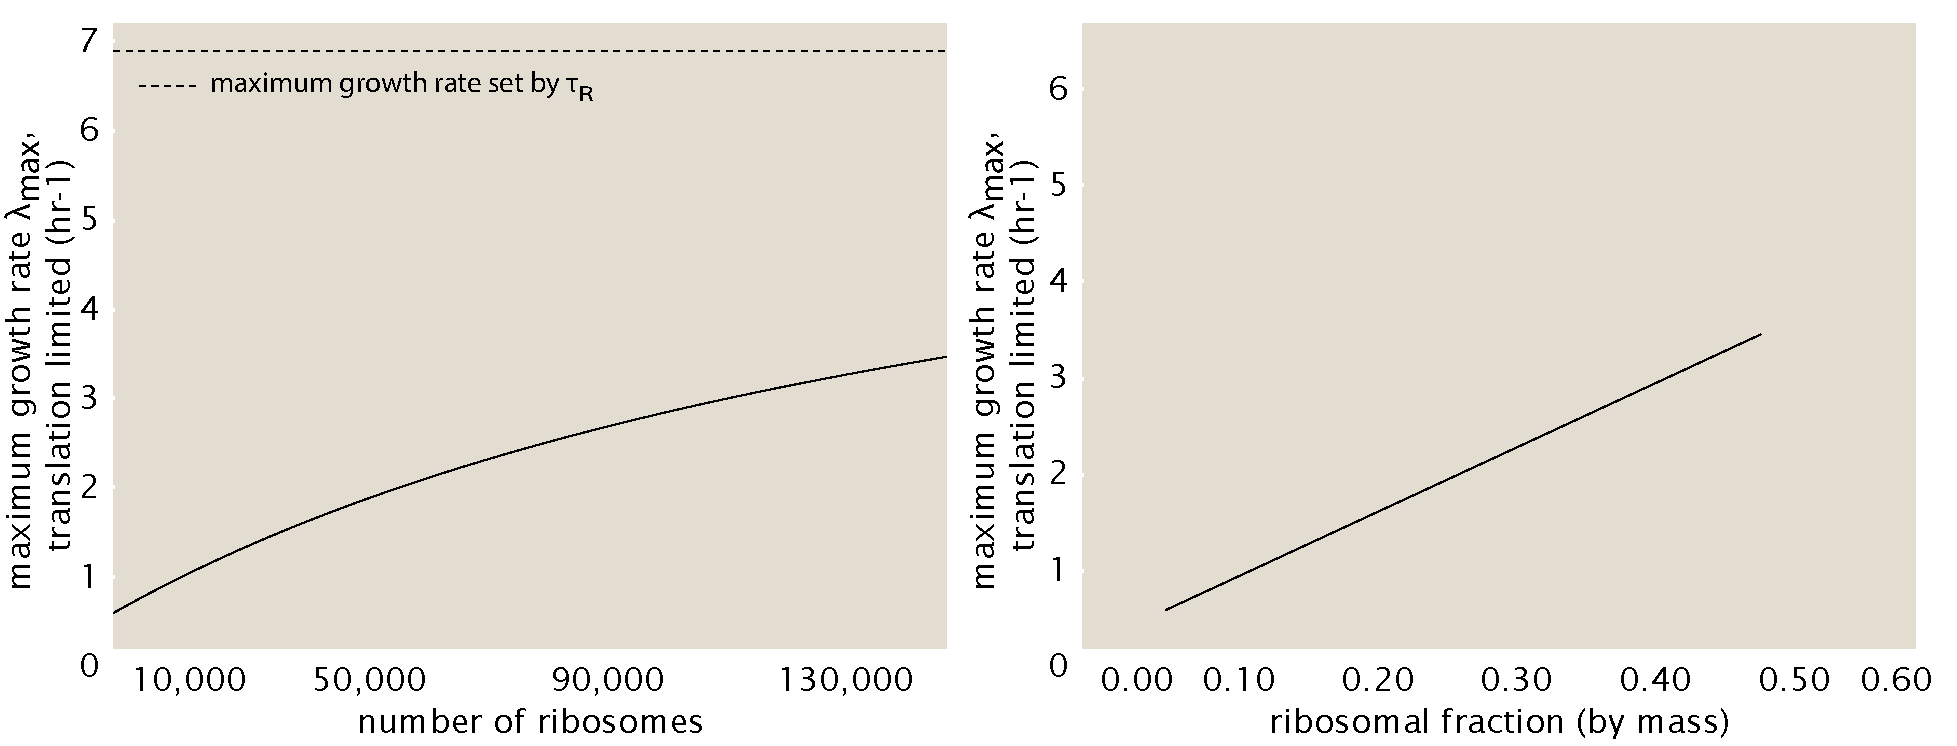
\includegraphics[width=1\textwidth]{../../code/figures/SI/estimates_translation_toy_1.pdf}
  \caption{{\bf Expectations on the maximum growth rate as a function of ribosome abundance.}
	 	A) Plot of the translation-limited growth rate in Equation
	 	\ref{eq:lambda_max}, with $N_{aa}$ = 1.2 x 10$^9$ amino acids, and $R$ from about
	 	10,000 to 150,000 copies per cell. B) Related to part A, but instead
	 	showing the translation-limited growth rate as a function of ribosomal mass
	 	fraction.}
  \label{fig:estimates_translation_toy_1}
\end{figure}

Given how many ribosomes a cell would need in order to double a cell in 6 minutes,
it is also useful to consider what this might mean with
respect to cell size. Note that cell volume will be proportional to cell mass.
We can estimate a lower bound on the required cell volume as a function of the
$R$ by assuming a mass density of 1.1 g/ml, and a dry mass of 30\% consisting of
only protein and RNA. This is plotted in Figure
\ref{fig:estimates_translation_volume}, where we've extended the range of $R$ up
to about one million copies per cell. While we find cell volumes consistent with our expectation for {\it E. coli}
for values of $R$ less than about 100,000 per cell, the plot also highlights that a cell would need to be
excessively largem with a minimal volume of about 25 $f$L, in order for
$\lambda_{\text{max}}$ to be close to the 6 minute doubling time set by the ribosome.

\begin{figure}[H]
		\centering
    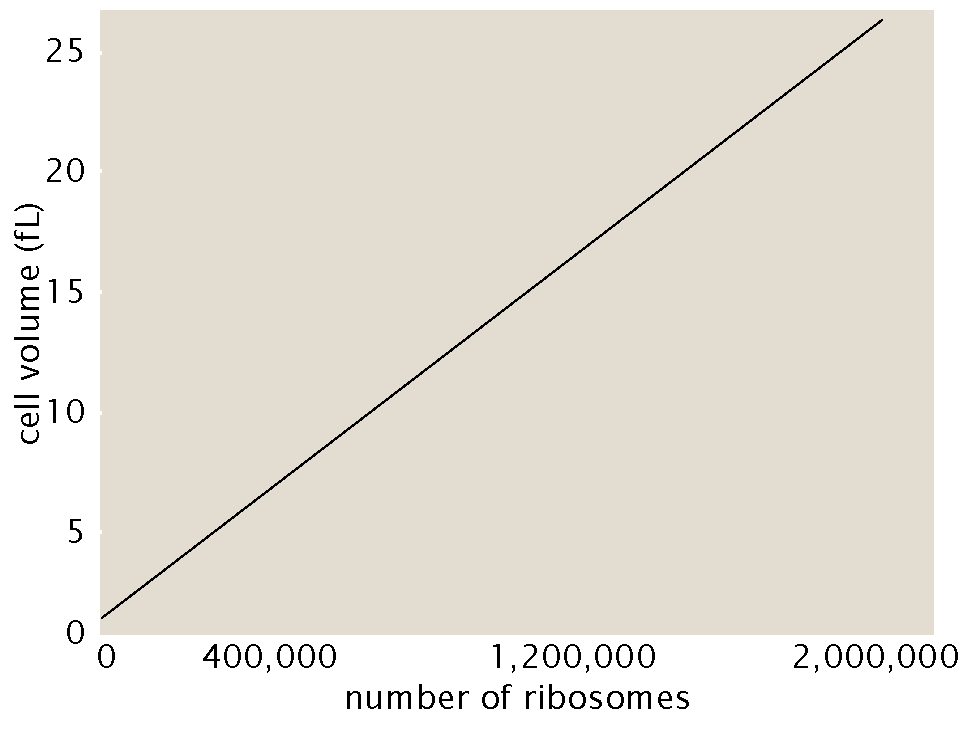
\includegraphics[width=0.5\textwidth]{../../code/figures/SI/estimates_translation_volume.pdf}
  \caption{{\bf Estimated scaling of cell size with ribosomal copy number.} As a first approximation,
	the cell mass it taken to consist of 214 fg non-ribosomal protein, and a ribosomal mass based
	on 1/3 corresponding to protein, and 2/3 corresponding to RNA. The cell volume is then calculated assuming
	a 30 \% dry mass, and cell mass density of 1.1 g/ml. }
  \label{fig:estimates_translation_volume}
\end{figure}

As a last consideration, one additional observation from Figure \ref{fig:estimates_translation_toy_1}B
is an apparently linear dependence
between $\lambda_{\text{max}}$  and the fraction of ribosomal mass. This, along with the
scaling in ribosomal copy number, are particularly relevant to the
phenomenological growth laws reported by others on how cell size and cell mass
scale with growth rate in bacteria. The linear scaling appears to be a feature
irrespective of the size of the non-ribosomal mass, as shown in Figure
\ref{fig:estimates_translation_ribo_frac}. Indeed, with a bit of algebra, we can
re-write the translation-limited growth rate defined by Equation
\ref{eq:lambda_max} as a function of ribosomal mass fraction, denoted by
$\Phi_R$, as,

\begin{equation}
\lambda_{\text{max}} =  \frac{ln(2)} {L_R} \cdot r_t \cdot \Phi_R.
\label{eq:lambda_max_phi}
\end{equation}
$L_R$ refers to the number of amino acids that make a single
ribosome ($L_R$ = 7,459 aa for a complete ribosome in {\it E. coli}). As a sanity check, we can quickly
see that if $\Phi_R$ = 1, we are once again limited only by the time required to
double a ribosome $L_R / r_t$.

\begin{figure}[H]
		\centering
    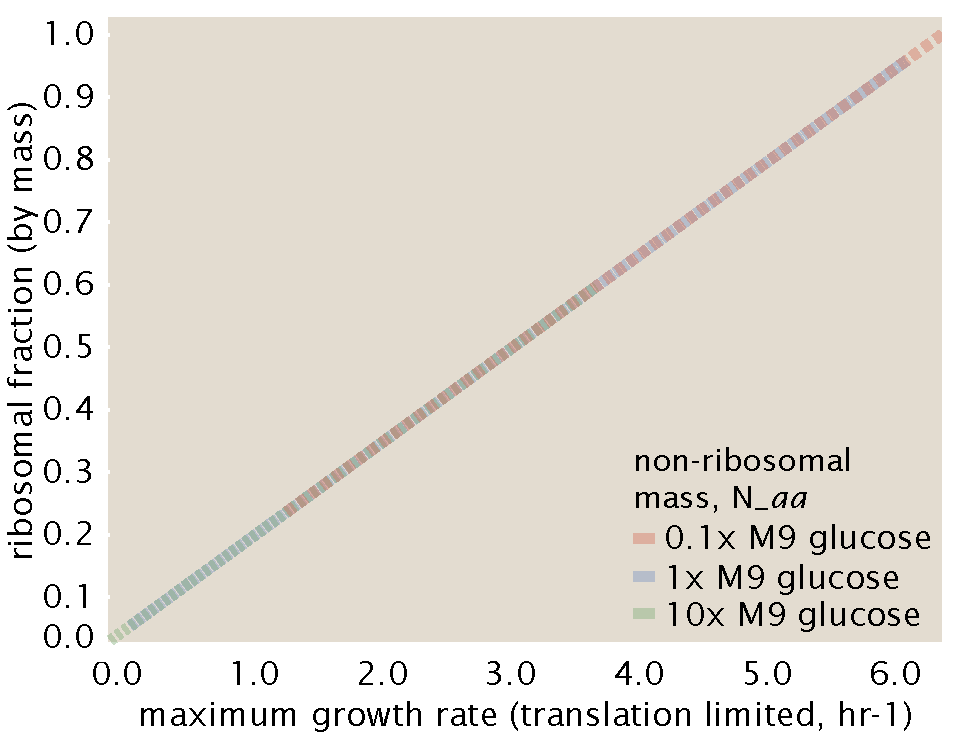
\includegraphics[width=0.5\textwidth]{../../code/figures/SI/estimates_translation_ribo_frac.pdf}
  \caption{{\bf Effect of ribosomal mass fraction on translation-limited growth rate.} Following the approach
	result from Figure \ref{fig:estimates_translation_toy_1}B, we recalculate the maximum growth rate as
	the total non-ribosomal mass is either reduced or increased ten-fold (i.e. $N_{aa}$ = [0.1x$N_{aa}$, $N_{aa}$, 10x$N_{aa}$]).}
  \label{fig:estimates_translation_ribo_frac}
\end{figure}


\subsection{Growth only appears translation-limited in rich growth media.}

With an expectation on the maximum growth rate achievable as a function of
ribosomal content from our discussion above, lets now take a look at our experimental
data. From Equation \ref{eq:lambda_max_phi}, we found that the
translation-limited growth  rate is simply determined by the fractional
ribosomal mass $\Phi_R$ which we can easily calculate from our proteomic data.   In Figure
\ref{fig:estimates_translation_data}A we plot this maximal growth rate,
$\lambda_{\text{max}}$, against the measured growth rates, while in Figure
\ref{fig:estimates_translation_data}B we plot the cell cycle or doubling time that would be
associated with these growth rates. The shaded regions identify regions that
should not be attainable with a translation elongation rate $r_t$ of 20 aa/s.
From these two plots, it appears that cells are only translation-limited in rich
media (data points with growth rates greater than $\approx$ 1 hr$^{-1}$ in Figure
\ref{fig:estimates_translation_data}A)).

% \marginnote{\small{NB: A better way would be to directly calculate the number of
% aa from proteomic sequences and copy number.}}

% \marginnote{\small{NB: There is something weird about the fraction of ribosomal
% protein in Peebo, Valgepea; it is higher, and also higher than that found in Scott
% {\it et al.}  - is it real??}}

\begin{figure}[H]
		\centering
    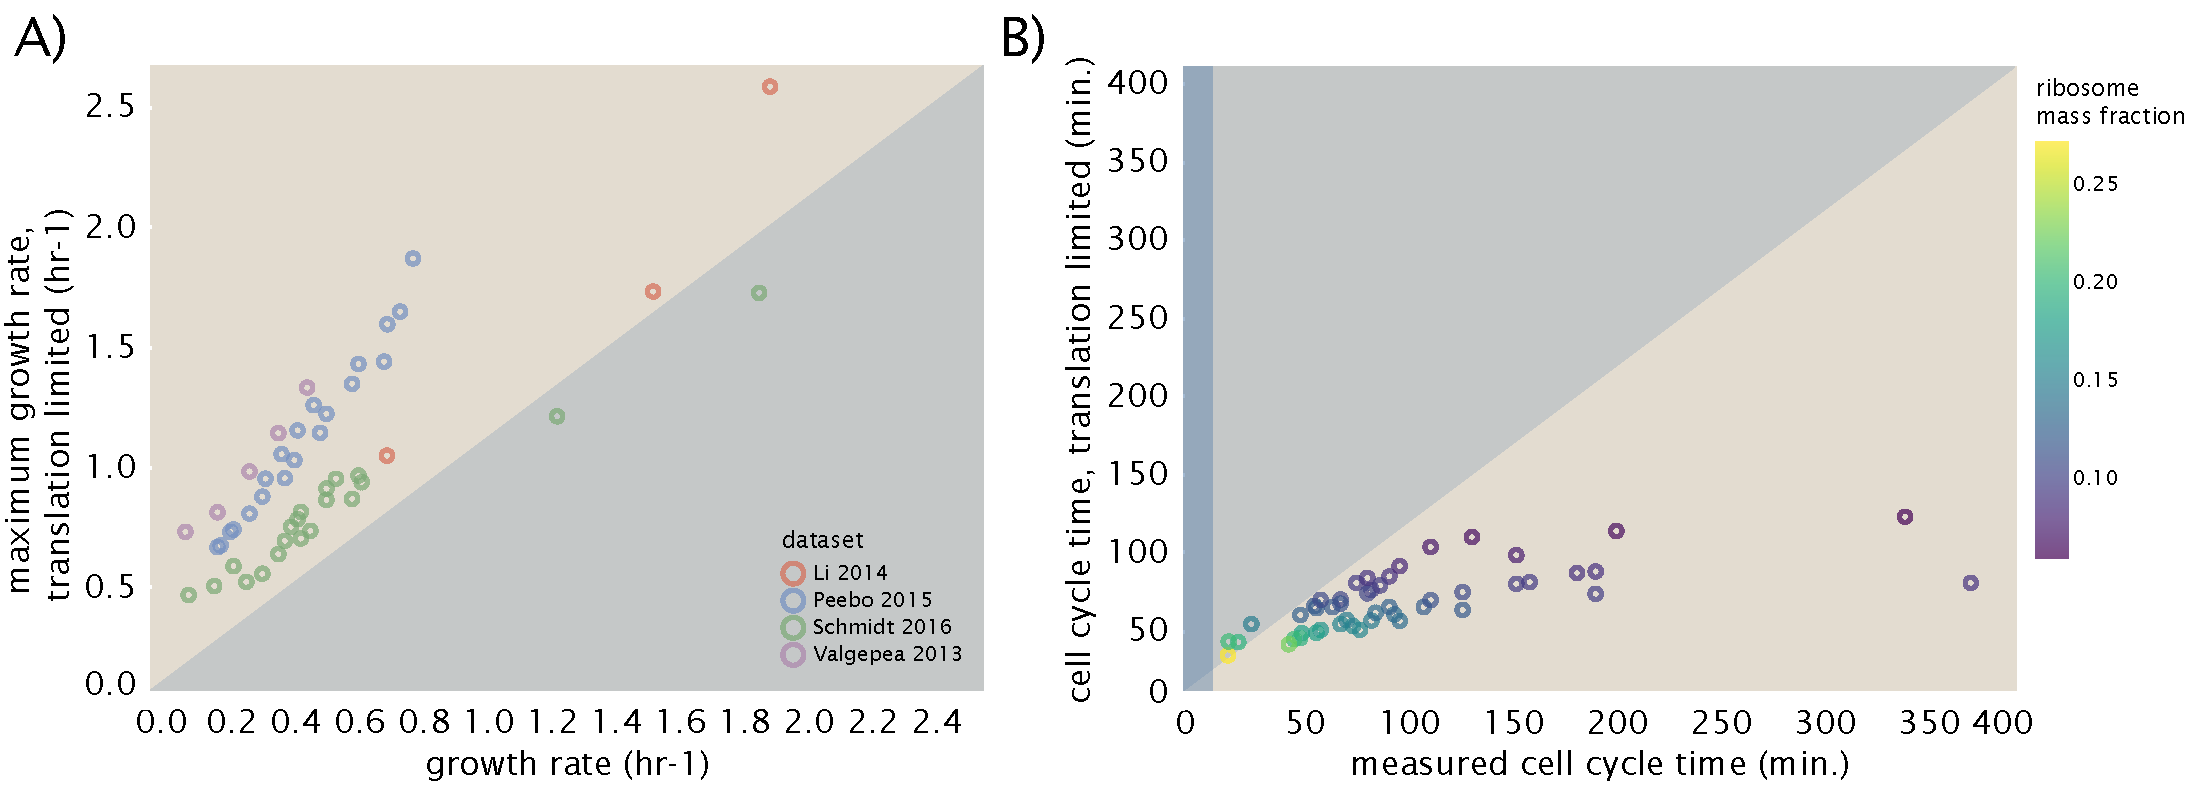
\includegraphics[width=1\textwidth]{../../code/figures/SI/estimates_translation_data.pdf}
  \caption{{\bf Comparison of translation-limited rate of growth to observed growth rates.}
	A) Plot of maximum growth rates based on reported cell mass and calculated from Equation \ref{eq:lambda_max}.
	B) Related to (A), but instead plotting the cell cycle time in minutes.
	The light shaded regions in (A) and (B) reflect boundaries where growth would not be possible
	due to a translation rate of 20 aa/s. The dark shaded region in (B) corresponds to the maximum
	division rate set by doubling a ribosome.
	(\smaller{NB: There is something weird about the fraction of ribosomal
	protein in Peebo, Valgepea; it is higher, and also higher than that found in Scott
	{\it et al.}  - is it real??})}
  \label{fig:estimates_translation_data}
\end{figure}

\subsection{The effect of a non-constant translation elongation rate.}

From Figure \ref{fig:estimates_translation_data}B it is apparent that for cells
with slower growth, the cell cycle time is indeed much longer than might have
been expected under translation-limited growth. The remaining parameter we have yet to
consider is the elongation rate $r_t$, which we have assumed to be 20 aa/s. Recent
measurements of elongation rate from Dai {\it et al.} \cite{Dai2016} across a
wide range of growth rates found that it indeed varies with growth rate. In particular,
they showed that the rate decreased to as low as 8 aa/s and exhibited a a Michaelis–Menten dependence on the
ribosomal fraction. Here we use their result to further consider the consequence of a
decreasing elongation rate $r_t$ on the maximum predicted growth rate.

% We can actually infer what
% the effective translation is given the observed growth rates, which we show
% in Figure \ref{fig:estimates_translation_rate}.  Interestingly, these
% translation rates are in good agreement with those measured in Dai {\it et al.}
% \cite{Dai2016}, which were also shown to decrease when grown under limited nutrient conditions.
%
% \marginnote{\small{JT suggests using measured elongation rate in Dai {\it et al.} to redefine
% translation boundaries in Figure \ref{fig:estimates_translation_data}.}}
%
% \begin{figure}[H]
% 		\centering
%     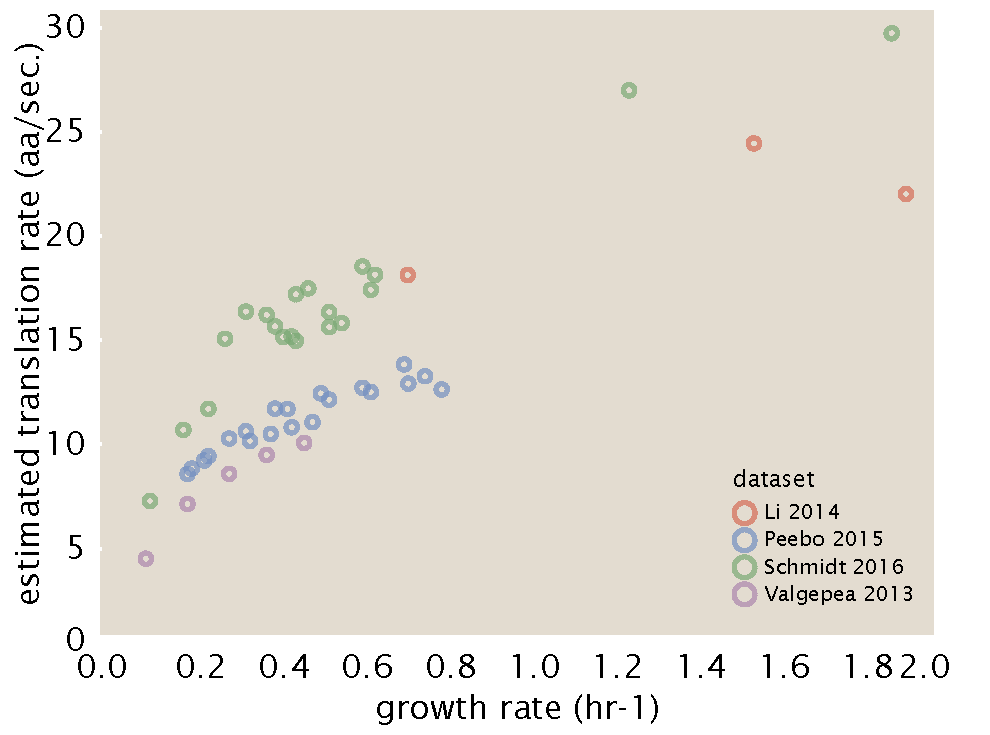
\includegraphics[width=0.5\textwidth]{../../code/figures/SI/estimates_translation_translation_rate.pdf}
%   \caption{{\bf Estimate of apparent translation rates based on observed growth rates and measured proteomic mass.}
% 	Using the measured ribosomal and non-ribosomal mass, we use Equation \ref{eq:lambda_max}  to estimate $r_t$
% 	for each of the proteomic datasets available.}
%   \label{fig:estimates_translation_rate}
% \end{figure}

\marginnote{\small{NB: a better approach would be from
point-of-view of biological rate-limiting steps. BUT the result suggests possibilities: aa-tRNA availability?,
GTP?}}

In the work of Dai et al. the authors propose that there may be a bottleneck in
translation that arises due to lower  availability of ternary complex (TC)
that must bind the ribosome in order for translation to proceed. This complex
consists of aminoacyl-tRNA, elongation factor Tu and guanosine triphosphate.
To account for this bottleneck, they divide the elongation rate into two
coarse-grained timescales: A) binding of the ternary complex to the ribosome,
which will depend inversely on the effective TC concentration $[TC_{eff}]$, and
B) other enzymatic processes that will not depend
on TC concentration. Letting these two timescales be 1/($k_{on} \cdot
[TC_{eff}]$) and 1/$r_t$, the new elongation rate is given by,

\begin{equation}
\frac{1}{r_t'} = \frac{1}{k_{on} \cdot [TC_{eff}]} + \frac{1}{r_t}
\label{eq:rate_dai}
\end{equation}
where $r_t/k_{on}$ is the binding constant of the TC with the ribosome. Further
taking $[TC_{eff}]$ to be proportional to the RNA/protein ratio,

\begin{equation}
[TC_{eff}] = C \cdot (R_m/P_m),
\label{eq:elong_rate}
\end{equation}
they find that  $r_t$ = 22 aa/s, $k_{on}$ = 6.4 $\mu M^{-1}s^{-1}$, and
$C$ = 31 $\mu M$.

\marginnote{\small{This assumption of proportionality
is something that will need some more consideration.}}

Using the elongation rate calculated from Equation \ref{eq:elong_rate}, we can now
recalculate the translation-limited growth rate,

\begin{equation}
\lambda_{\text{max}}' =  \frac{ln(2)} {L_R} \cdot r_t' \cdot \Phi_R,
\label{eq:lambda_max_phi_dai}
\end{equation}
where we denote $\lambda_{\text{max}}'$ as the translation-limited growth rate when elongation rates is no longer assumed
to be fixed at 20 aa/s. Plugging in the translation rate $r_t'$ given by Equation \ref{eq:rate_dai}
along with the measured fraction of ribosomal mass $\Phi_R$ from each dataset, we find a
further improvement in agreement between the measured and translation-limited growth rates.
This is shown in Figure \ref{fig:estimates_translation_data_dai}. This is particularly true with
the data from Li {\it et al.} and Schmidt {\it et al.}, though we note that
for the poorest nutrient conditions (i.e. the longest cell cycle time) a
discrepancy still appears to exist.

\begin{figure}[H]
		\centering
    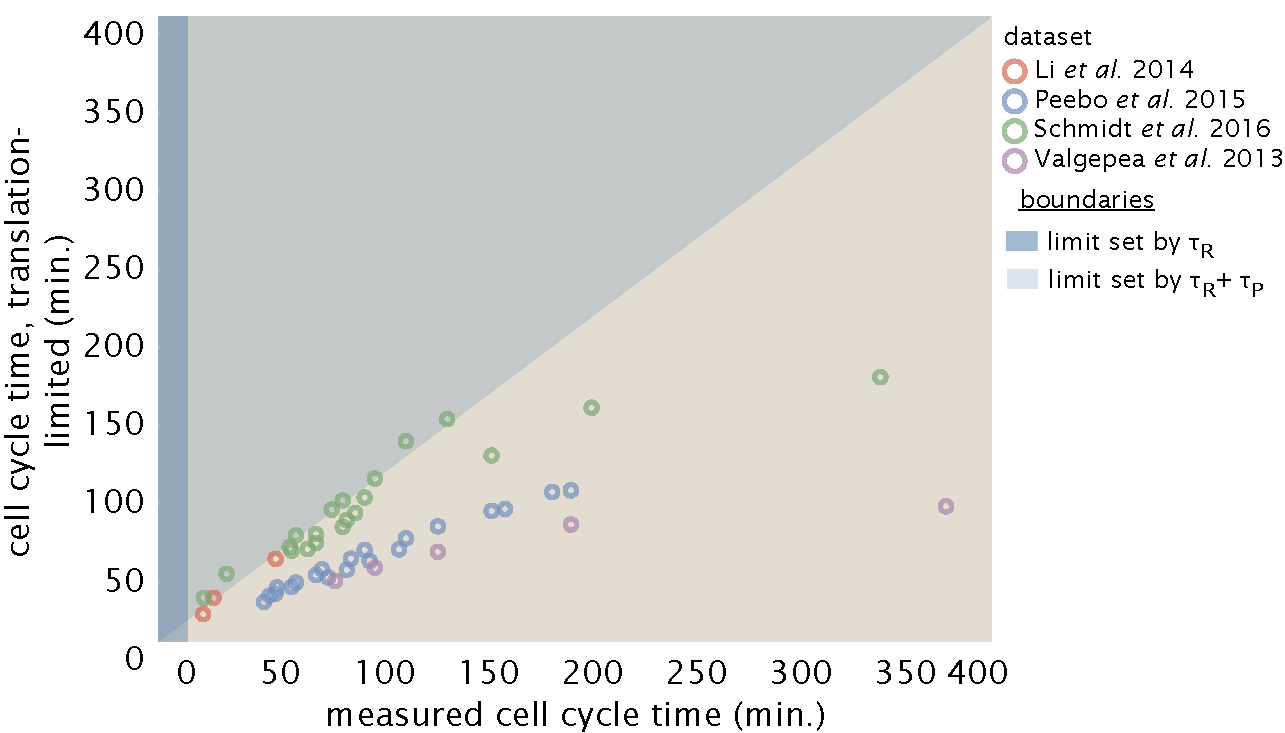
\includegraphics[width=0.7\textwidth]{../../code/figures/SI/estimates_translation_data_dai.pdf}
  \caption{{\bf Comparison of translation-limited rate of growth to observed growth rates using the predicted
	elongation rate from Dai {\it et al.}.}
	Predicted cell cycle time, calculated from  Equation \ref{eq:lambda_max_phi}, is plotted
	against the measured doubling time.	The light shaded region reflect a boundary where growth would not be possible
	given the predicted translation rate $r_t'$ in Equation \ref{eq:rate_dai}, which varies from about 8 aa/s to about 20 aa/s.
	The dark shaded region corresponds to the maximum
	division rate set by the synthesis of a ribosome. To calculate the RNA/ protein ratio
	$R_m/P_m$ we assume it is proportional to the fraction of ribosomal mass $\Phi_R$,  which
	empirically was found to be $R_m/P_m$ = $\Phi_R$/0.411 \cite{Dai2016}.}
  \label{fig:estimates_translation_data_dai}
\end{figure}



\newpage
\section{Nutrient-dependent limits on the rate of cell division.}

% Consider starting by showing the data from Dai et al. and propose alternative
% explanation.

In the preceeding section we identified limitations on the speed of cell
division that reflect inherent limits on the maximum translation elongation rate
and the necessity to double both the pool of ribosomes and the cell's remaining
proteome. We next consider the conseqences of nutrient limtations on the maximal
growth rate of the cell.

Here it is helpful to point out three notable experimental observations.  The
first is that in the limit of zero growth, the ribosomal fraction of {\it E.
coli} converges toward nonzero value (5-10 \% by mass). In the context of poorer
and poorer nutrient conditions, there must be a point in which cells have more
ribosomes than they can utilize. The next point, which is related to this,  is
that cells actually appear to reduce the fraction of ribosomes that are actively
translating when growing at a growth rate less than 0.7 hr$^{-1}$. Lastly, below this
growth rate, the cell's elongation rate also begins to decrease, with a minimum value of about 8
aa/s measured in stationary phase.

% only drops to aboutapproximately 8 aa/s. From
% Figure XB, we can see that that only way for a cell  to grow faster at an
% elongation rate of 8 aa/s is to increase its ribosomal fraction.

% The last point
% is that a single {\it E. coli} cell in limiting nutrient conditions still has
% about Z fg total protein,  as well as DNA, RNA, lipid, etc. whose quantities
% must all be doubled. Behind this last observation is a somewhat subtle but
% important point that the absolute  abundances that enable it to be a living
% organism must also be considered. This last point  provides us with an
% additional constraint on growth that becomes important in the nutrient-dependent
% limit and we consider this further in the next section.

\subsection{Nutrient limitation does not explain increasing ribosomal content.}

We begin by considering the consequence of nutrient limitation on the ribosomal elongation rate. In the
work of  Dai {\it et al.} it was suggested that perhaps there is a bottleneck in
the availability of ternary complex, referring to the assembly of
aminoacyl-tRNA,  elongation factor Tu and guanosine triphosphate (GTP) that is
needed for translation.  If cells are indeed  reducing their fraction of
actively translating ribosomes, it is difficult to rationalize the possibility
that a protein like Tu might be limiting. If it were limiting, for example, a
simple solution seems to be for the cell to make  fewer of the unused ribosomes
and increase the number of Tu. In contrast, at least in the limit  of poorer
nutrient conditions, the possibility of limitations on more basic building blocks like amino
acids  and GTP seem more reasonable. Here we consider the possibility that the
synthesis rate of  amino acids, and therefore the cellular concentration of
amino acids $[aa]$ is limiting. An important finding from our analysis below is
that while we are able to account for both the change in translation rate and
the apparent fraction of ribosomes that are needed for a specific growth rate, it provides no
basis to explain why ribosomal content continues to increase as growth rate increases.

In order to consider that the amino acid synthesis rate is limiting, we can
follow a similar approach to that employed by Dai et al., which was to divide
the elongation rate into two coarse-grained timescales. Here we assume that  the
translation rate depends on A) binding of a ternary complex, which we propose
depends on a rate-limiting concentration of $[aa]$ and, 2) other enzymatic
processes that will not depend on $[aa]$. The effective elongation rate is given
by the inverse timescales associated with each step,

\begin{equation}
\frac{1}{r_t'} = \frac{1}{k_{on} \cdot [aa]} + \frac{1}{r_t}.
\label{eq:rate_dai_2}
\end{equation}
where $r_t'$ is the measured elongation rate, $r_t$ is the maximum elongation
rate, and $r_t/k_{on}$ is the binding constant $K_d$ of the ternary complex with
the ribosome. Alternatively, we can re-write this in terms of the binding
constant,

\begin{equation}
r_t' = r_t \cdot \frac{1}{1 + K_d / [aa]}.
\label{eq:rate_aa}
\end{equation}
If we consider only consumption of amino acids by ribosomes, during steady state growth $[aa]$ will be depend on the amino
acid synthesis rate $r_{aa}$, consumption rate by ribosomes, $R \cdot r_t'$,  and the cell volume $V$,

\begin{equation}
[aa] =  \tau \cdot \frac{r_{aa} - R \cdot r_t'}{V}.
\label{eq:aa}
\end{equation}
Here $\tau$ refers to the doubling time of the cell in seconds. If we plug this into Equation \ref{eq:rate_aa}, we find that

\begin{equation}
r_t' = r_t \cdot \frac{1}{1 + K_d \cdot V / (\tau \cdot (r_{aa} - R \cdot r_t'))}.
\label{eq:rate_aa_2}
\end{equation}
This brings us to a somewhat confusing result. If ribosomes are in excess of the
available amino acids, ribosomes will deplete the supply of amino acids and
translation will grind to a halt. This apparent conundrum seems to be
similarly present if we were to instead consider that the supply of tRNA or GTP is
limiting. This may provide some rationalization for why a cell would
regulate its fraction of active ribosomes.

In order to proceed, we will take for granted that the cell actively regulates
its fraction of active ribosomes, and make an assumption that it does so to
support a net positive concentration of amino acids in the cell. Specifically, we are
interested in how the elongation rate might depend on a positive increase in the
synthesis rate of amino acids. Here we re-write Equation
\ref{eq:rate_aa_2} as,

\begin{equation}
r_t' = r_t \cdot \frac{1}{1 + K_d' / r_{aa}'},
\label{eq:rate_aa_3}
\end{equation}
where $r_{aa}'$ is the effective rate in which amino acid are being supplied to
each of the active ribosomes, and $K_d'$ is the apparent rate when $r_t'$ is
half maximal. Here $K_d' = K_d \cdot V / \tau$, while $r_{aa}' = r_{aa} - R \cdot
r_t'$.

With a maximal elongation rate of about 17 aa/s, we find that for any $K_d'$
less than 8.5 aa/s, the time to double the  cell's proteome will be limited by
$r_{aa}'$, and not the elongation rate $r_t$. Said differently, if
the total number of amino acids consumed to double the cell is $N_aa$, it
should take $\tau = N_aa/r_{aa}'$ to double the cell, which is less than the time
required if all ribosomes were constantly synthesizing proteins at their rate of $r_t'$.
Under such a scenario, the fraction of available ribosomes that are  needed would just be given
by the ratio of  $r_{aa}'/r_t'$.

In Figure \ref{fig:aa_limitation_2}(A) we consider such a scenario and consider the growth rate of cells
as the value of $r_t'$ is increased from 2 - 50 aa/(s ribosome). Here we have selected a value of
$K_d'$ less than 8.5 aa/(s ribosome), with a cell containing 7\% ribosome by mass.  Since we are considering cells growing in steady
state, and we assume  that the cell has some mechanism in place to match a
specific supply of amino acids defined by  $r_{aa}'$,  the fraction of available
ribosomes needed to double the cell will be given by $r_{aa}'/r_t' $, up to a maximum value of 1.
This is plotted in Figure \ref{fig:aa_limitation_2}(B).

\begin{figure}[H]
		\centering
    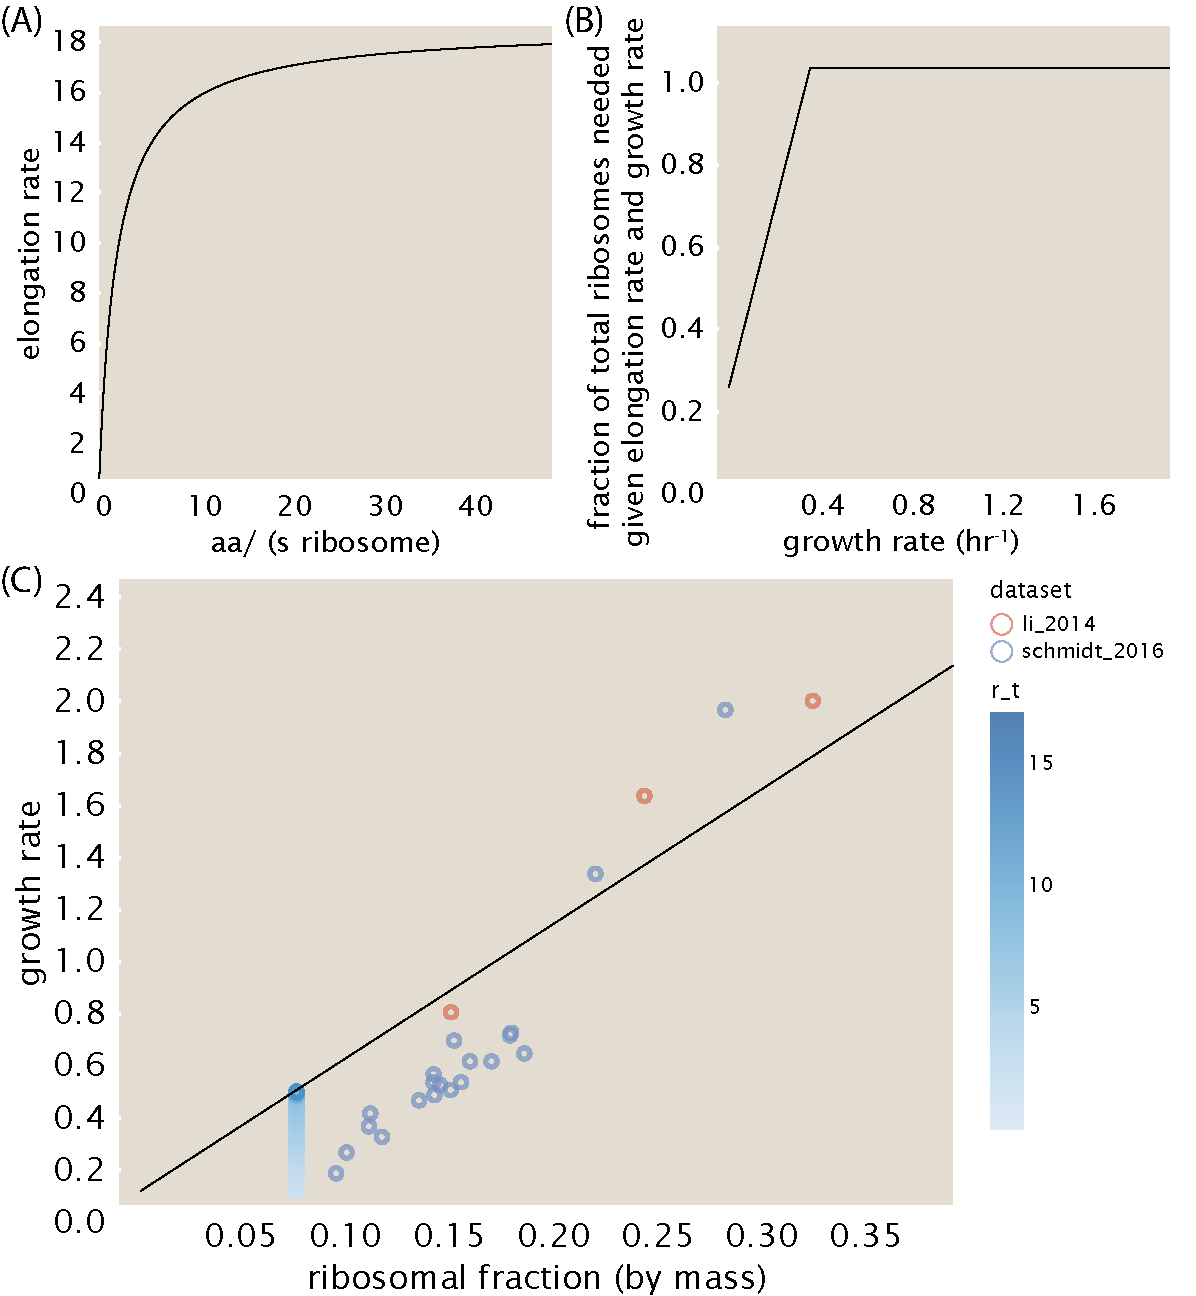
\includegraphics[width=0.9\textwidth]{../../code/figures/SI/aa_limitation_2.pdf}
  \caption{{\bf Expectations on cell growth in a nutrient-limited regime.}
	(A) Plot of elongation rate $r_t$ using Equation \ref{eq:rate_aa_3}, with  $K_d'$
	less than 8.5 aa/(s ribosome). (B) The apparent fraction of ribosomes that would be needed
	given that the supply of amino acids $r_{aa}'$ is less than the rate with which
	ribosomes are using them. We assume that cells are growing in steady state, and that the cell is
	able to regulate its fraction of ribosomes in order to maintain a constant supply of amino acids $r_{aa}'$ . (C) Plot of growth rate versus ribosomal fraction. Blue line
	refers to a cell whose ribosomal fraction in limiting growth is 7 \%, with the color indicating
	the elongation rate as production rate of amino acids $r_{aa}'$ is increased over the range shown
	in part (A).  }
  \label{fig:aa_limitation_2}
\end{figure}

Importantly, while this provides some perspective on why elongation might decrease in the nutrient limit,
and can be consistent with apparent regulation of the active pool of ribosomes. However, as shown in
Figure \ref{fig:aa_limitation_2}(C) it does so
without requiring any increase in ribosomal
content as a function of growth rate. This suggests that something else must be considered in order to
explain the observedtrend in ribosomal present that is still observed in the nutrient-limit.


% This provides an interesting rationalization of why a cell
% might actively regulate its fraction of active ribosomes. Specifically, while
% amino acid synthesis rate is below its consumption rate, the excess ribosomes
% would otherwise consume the available pool of amino acids and bring elongation
% to a halt. It would also be impossible to distribute the supply of 20 distinct
% amino acids as protein synthesis proceeds.

\newpage

\subsection{Nutrient limitations provide another boundary on the rate of
bacterial growth.}

As an {\it E. coli} cell encounters more nutrient rich conditions, the data in
Figure XA shows that the measured steady state growth rates follows a
well-defined path as a function of ribosomal content. This reflects the
so-called growth law that has been observed for {\it E. coli} and some other
bacterium. However, we might have naively expected alternative paths to reach
the translation-limited growth  boundary  to be equally plausable. In order to
make progress it useful to highlight that experimentally, from work by Dai {\it
et al} and others, the elongation rate is expected to increase gradually
from about 8 aa/s to a maximum in rich media of about 17 aa/s.

To understand the consequence of this, we consider the hypothetical situation
illustrated in Figure Z. Here a cell is initially growing at a rate of about X
hr$^{-1}$, with an  elongation rate of X aa/s. As nutrient conditions improve
and the apparent elongation rate  increases, the maximum growth rate becomes
defined by this new elongation rate. The first  naieve scenario is that the
bacterium keeps its proteome unchanged, including the  number of available
ribosomes. Such a situation would correspond to a cell whose size  and total
contents can remain unchanged and it can just double itself faster. The  second
scenario is that the cell takes advantage of its apparent increase in protein
synthesizing  capacity, and somehow bias its protein production to make more
ribosomes. By doing so, the cell is able to grow faster given its new elongation
rate.

We next attempt to estimate the additional ribosomes than might be made from
this additional capacity. This can be determined from the relative increase in
elongation rate and the number of available ribosomes. The additional amino
acids available to put toward making more proteins is given by,

\begin{equation}
	N_{aa}' = (r_{t 16} - r_{t 14}) \cdot \tau \cdot R,
\end{equation}
where $\tau$ is the doubling time of the cell. The maximum additional ribosomes
than can then be made is simply given by,

\begin{equation}
 R' = N_{aa}' / L_R,
\end{equation}
where again, $L_R$ refers to the total number of amino acids that make a
ribosome. This scenario results in a cell with larger ribosomal fraction given by,

\begin{equation}
 \Phi' = \frac{R + R'}{ R + R' + P' }.
\end{equation}
The maximal growth rate at this elongation rate will then be equal to
\begin{equation}
 \lambda = \frac{ln(2)}{ L_R} \cdot r_{t 16} \cdot \Phi'.
\end{equation}
While this treatment is somewhat artificial and assumes that the cell continues
to  double its core proteome, as measured in the slow-growth limit, it provides
us with a convenient way to rationalize the constantly increasing ribosomal
fraction for growth rates below the traslation-limited growth rate. Indeed,
since cells do indeed making more ribosomes and get more massive with growth
rate, this perspective provides an a potential way to connect to the
well-characterized cell size scaling observed in {\it E. coli}.

We can repeat the same thought process for the entire range of measured
elongation rates, from about 8 aa/s to 17 aa/s, which is plotted in Figure Z.
Here we now identify a nutrient-limited boundary. This boundary represents the
scenario where any increase in cell protein mass has been devoted to making more
ribosomes.

Here it is worth noting that this boundary isn't fundamentally as restricted as the
translation-limited boundary. For example, there are many examples from the Hwa
lab where the addition of an antibiotic like chloramphenicol shift the observed
ribsomal fraction and growth rates into this region.


%
% \subsection{Nutrient-limited building blocks and biased ribosome production.}
%
% Here we include our proposed dependence of translation elongation on the production rate of
% amino acids. Specifically, we look at how the growth rate increases as a function of
% amino acid production rate using our proposed scheme above.
%



\bibliography{exploring_translation_limits.bib}

\end{document}
